% Standalone copy of the TikZ flowchart on Lecture 4's "What Is a Decision Tree?" frame,
% for the Quarto mirror (browsers cannot show PDF, so the mirror uses decision_tree.svg).
% The block between the markers is copied VERBATIM from Slides/Lecture04_DecisionTrees.tex;
% the Beamer file is the source of truth. Rebuild after any change there:
%   latex -output-directory=<scratch> extract_tikz.tex          (DVI mode, not xelatex)
%   dvisvgm --no-fonts --bbox=papersize <scratch>/extract_tikz.dvi -o decision_tree.svg
\def\pgfsysdriver{pgfsys-dvisvgm.def}      % TikZ drawing as SVG paths
\documentclass[11pt, border=4pt]{standalone}
\usepackage{amsmath, amssymb}
\usepackage{xcolor}
\usepackage{tikz}
\renewcommand{\familydefault}{\sfdefault}   % Beamer: sans text, serif math
\definecolor{unocrimson}{HTML}{D71920}
\definecolor{unolightcrimson}{HTML}{FDECEA}
\definecolor{unogreen}{HTML}{15803D}
\definecolor{unolightgreen}{HTML}{F0FAF4}
\begin{document}
% ---- BEGIN verbatim from Slides/Lecture04_DecisionTrees.tex ----
    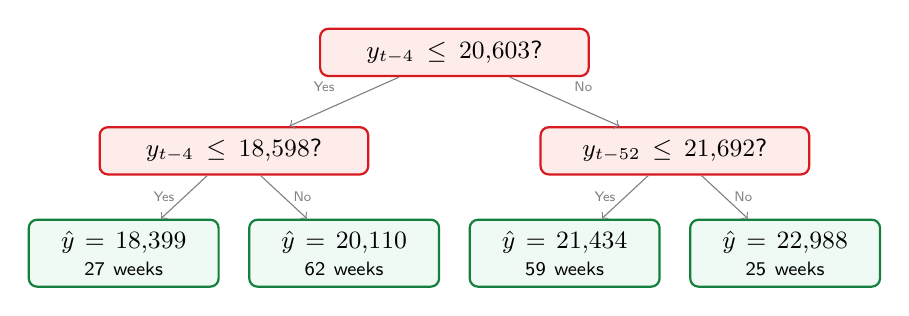
\begin{tikzpicture}[
      every node/.style={font=\small},
      internal/.style={rectangle, rounded corners=3pt,
        fill=unolightcrimson, draw=unocrimson, line width=0.8pt,
        align=center, inner sep=3pt, text width=3.2cm,
        minimum width=3.4cm, minimum height=0.6cm},
      leaf/.style={rectangle, rounded corners=3pt,
        fill=unolightgreen, draw=unogreen, line width=0.8pt,
        align=center, inner sep=3pt, text width=2.2cm,
        minimum width=2.4cm, minimum height=0.85cm},
    ]
      \node[internal] (root) at (4.9, 0)     {$y_{t-4} \leq 20{,}603$?};
      \node[internal] (l1)   at (2.1, -1.25) {$y_{t-4} \leq 18{,}598$?};
      \node[internal] (r1)   at (7.7, -1.25) {$y_{t-52} \leq 21{,}692$?};
      \node[leaf] (a) at (0.7, -2.55) {$\hat{y} = 18{,}399$\\[-1pt]{\scriptsize 27 weeks}};
      \node[leaf] (b) at (3.5, -2.55) {$\hat{y} = 20{,}110$\\[-1pt]{\scriptsize 62 weeks}};
      \node[leaf] (c) at (6.3, -2.55) {$\hat{y} = 21{,}434$\\[-1pt]{\scriptsize 59 weeks}};
      \node[leaf] (d) at (9.1, -2.55) {$\hat{y} = 22{,}988$\\[-1pt]{\scriptsize 25 weeks}};
      \draw[->, gray] (root) -- (l1) node[midway, above left, font=\tiny]{Yes};
      \draw[->, gray] (root) -- (r1) node[midway, above right, font=\tiny]{No};
      \draw[->, gray] (l1) -- (a) node[midway, left, font=\tiny]{Yes};
      \draw[->, gray] (l1) -- (b) node[midway, right, font=\tiny]{No};
      \draw[->, gray] (r1) -- (c) node[midway, left, font=\tiny]{Yes};
      \draw[->, gray] (r1) -- (d) node[midway, right, font=\tiny]{No};
    \end{tikzpicture}
% ---- END verbatim ----
\end{document}
